\subsection{自由群}
\begin{prob}
证明$S_{4}$由元素$a,b$生成,而$a,b$适合$a^{2}=b^{3}=e,\left(ab\right)^{4}=e$。
\end{prob}
\begin{prob}
证明$A_{4}$由元素$a,b$生成,而$a,b$适合$a^{2}=b^{3}=e,\left(ab\right)^{3}=e$。
\end{prob}
\begin{prob}
设群$G$由元素$a,b$生成,有定义关系$a^{4}=b^{4}=e,a^{2}=b^{2},b^{-1}ab=a^{-1}$。证明$G$为第1章$\S 1.3$的习题$11$定义的8阶四元数群。
\end{prob}
\begin{prob}
设$F$是的自由群,$G,H$是群。设$\alpha :F\rightarrow G$是同态,$\beta :H\rightarrow G$是满同态,则存在同态$\gamma :F\rightarrow H$使得$\alpha =\beta \gamma $。(本习题的结论常称为是{\bfseries 自由群的万有性质}或{\bfseries 自由群的投射性质})
\end{prob}
\begin{figure}[h]
    \centering
    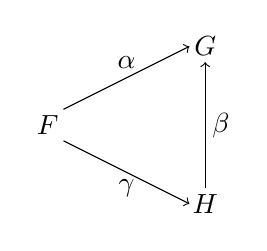
\begin{tikzpicture}
    \node at (0,0) {$F$};
    \node at (2,1) {$G$};
    \node at (2,-1) {$H$};
    \draw [->] (0.2,0.2) -- (1.8,1);
    \node at (1,0.8) {$\alpha $};
    \draw [->] (0.2,-0.2) -- (1.8,-1);
    \node at (1,-0.8) {$\gamma $};
    \draw [->] (2,-0.8) -- (2,0.8);
    \node at (2.2,0) {$\beta $};
    \end{tikzpicture}
    \caption{第四题图}
\end{figure}